\section{Interconnect}
\label{sec:interconnect}

The T4 has no NVLink, so this half of the table has no published prior to
deviate from; whitepaper geometry (two NV2 links, ${\sim}50$~GB/s per
direction aggregate) supplies the sanity gates.

A pointer chase into the peer's memory costs 472~ns --- a 172~ns NVLink
hop over the local DRAM latency --- and the default and \texttt{.cg}
chases measure identically: peer lines do not enter the local L1 at all.
SM-path streaming sustains 43.4~GB/s reading and 45.8 writing per
direction (inside the $\pm15\%$ gate; posted writes faster), and a peer
\texttt{atomicAdd} chains at 541~ns. With one GPU streaming inbound
writes at full NVLink rate, the victim's local DRAM read bandwidth
degrades 15.1\% at the defined operating point.

The exchange primitive of \cref{sec:hyp-exchange} --- peer store,
\texttt{\_\_threadfence\_system} (which lowers to
\texttt{MEMBAR.SYS}+\texttt{CCTL}+\texttt{ERRBAR}), flag write, remote
spin and acknowledge --- round-trips between concurrently resident
kernels in 3.90~\textmu s empty, 4.92 at 4~KiB, and 7.94 at 20~KiB, with
a data-check litmus run before any timing is trusted. The NCCL
comparator, environment pinned (Ring, LL, two channels, NCCL 2.30.4),
holds a steady-state two-rank all-reduce floor of 21.1--28.3~\textmu s
across 4--64~KiB, with a cold first call in the milliseconds (5--10~ms
across four fresh-communicator samples; the row is flagged for its
spread); the in-situ production figure this study set out to explain is
retired in favour of these standalone numbers. PCIe rows complete the
picture: 12.2/13.2~GB/s pinned in each direction on both x16 GPUs, and a
${\sim}4$~\textmu s pinned small-transfer floor. \Cref{tab:interconnect}
collects the rows; \cref{fig:exchange} sets the primitive against the
registered bar of \cref{sec:hyp-exchange}.

\begin{table}[t]
\centering
\caption{Interconnect rows, GPU0$\to$GPU1 direction (the reverse
direction agrees within 1\% throughout). The cold NCCL row is the median
of four fresh-communicator samples spanning 5--10~ms and carries a
spread flag in the table.}
\label{tab:interconnect}
\small
% generated by tools/mk_paper_tables.py -- do not edit
\begin{tabular}{@{}l r@{}}
\toprule
quantity & value \\
\midrule
peer load latency (NVLink hop) & 472 ns \\
peer \texttt{atomicAdd} latency & 541 ns \\
peer read bandwidth & 43.4 GB/s \\
peer write bandwidth & 45.8 GB/s \\
\addlinespace
one-way message, flag only & 1.20 \textmu s \\
exchange round trip, flag only & 3.93 \textmu s \\
exchange round trip, 4 KiB & 4.91 \textmu s \\
exchange round trip, 20 KiB & 7.94 \textmu s \\
\addlinespace
NCCL all-reduce, 4 KiB steady & 21.1 \textmu s \\
NCCL all-reduce, 20 KiB steady & 25.0 \textmu s \\
NCCL all-reduce, first call (cold) & 8.14 ms \\
\addlinespace
PCIe 3.0 x16 pinned H2D / D2H & 12.2 / 13.2 GB/s \\
PCIe small-transfer floor (4 B H2D) & 3.89 \textmu s \\
\bottomrule
\end{tabular}

\end{table}

\begin{figure}[t]
\centering
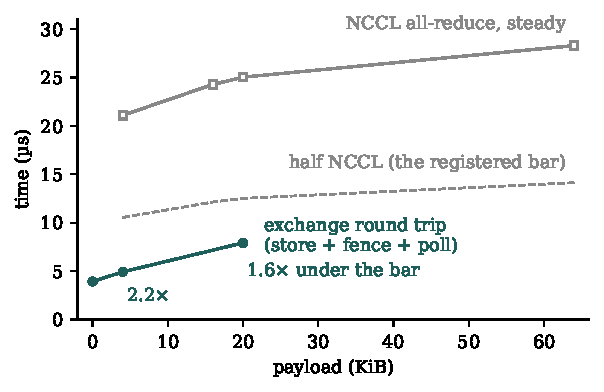
\includegraphics{figures/fig_exchange}
\caption{The exchange primitive against the NCCL per-call floor. The
registered comparison applies where the composed-prediction gate passes
(4~KiB and below); at 20~KiB the margin is observational
(\cref{sec:hypotheses-outcomes}).}
\label{fig:exchange}
\end{figure}
